\subsection{\Glsfmtlong{td}}\label{subsec:wottd}

Die \glsfirst{td} \autocite{w3c.wot.td.20200623} hat, wie in \autoref{subsec:wotarchitecture} bereits oberflächlich beschrieben, vier Hauptbestandteile:

\begin{itemize}
  \item Beschreibende Metadaten über das \gls{thing};
  \item Interaktionsaffordanzen, die beschreiben, wie man das \gls{thing} nutzen kann;
  \item Schemata, die beschreiben, wie die Daten aussehen (müssen), die entweder an das oder von dem \gls{thing} geschickt werden;
  \item Verweise auf verwandte \glspl{thing} oder Dokumente.
\end{itemize}

Eine \gls{td} wird in \glsxtrshort{json} verfasst und folgt dem \glsxtrshort{jsonld}-Standard. Dabei existieren verschiedene Vokabulare für die unterschiedlichen Bereiche des Informationsmodells, die als Kontext verwendet werden können.

Jedes Vokabular enthält im Grunde Definitionen von Datenstrukturen, die im objektorientierten Kontext als Objekte verstanden werden können. Das Kernvokabular definiert dabei den grundsätzlichen Aufbau einer \gls{td}, während es dabei die anderen spezifischeren Vokabulare für ihre jeweiligen Teilbereiche referenziert.

\subsubsection{Kernvokabular}

Das Kernvokabular deckt das Interaktionsmodell aus Eigenschafts-, Aktions- und Ereignisinteraktionsaffordanzen ab.

\begin{figure}[H]
  \centering
  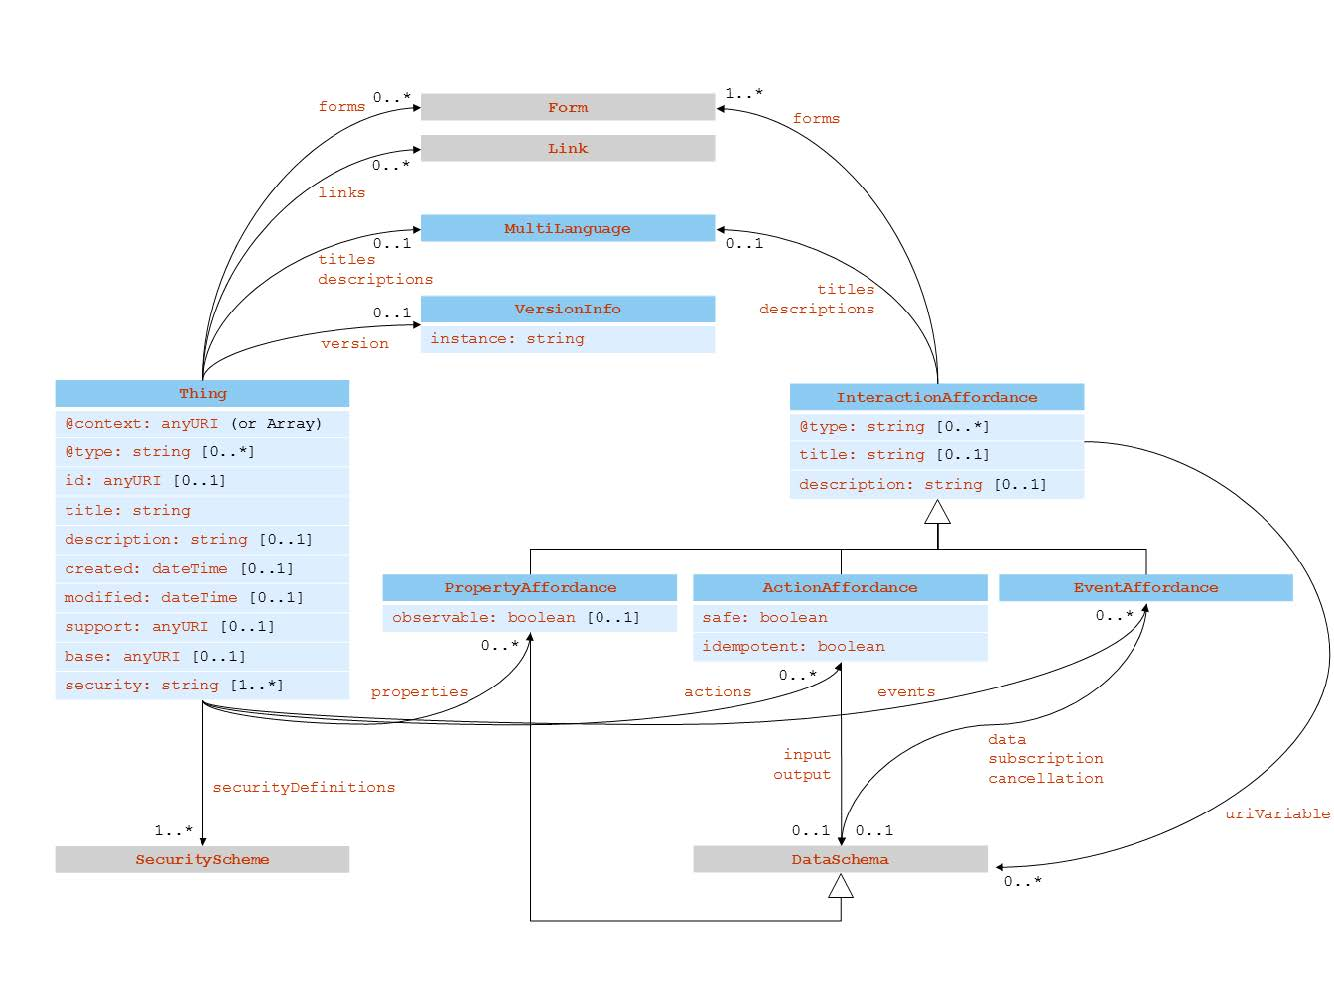
\includegraphics[width=\textwidth]{td-core-vocabulary.jpg}
  \caption{\glsxtrshort{td} Kernvokabular}\label{fig:td_core_vocabulary}
\end{figure}

Das \lstinline{Thing} ist dabei das Grundobjekt, welches die Wurzel eines \glsxtrshort{td}-Dokuments definiert. Dazu gehören der \gls{uri} des \gls{thing}[s], \glsxtrshort{jsonld}-Annotationen, Beschriftungen, Metadaten, vor allem aber die einzelnen Bereiche des Interaktionsmodells, Links zu anderen \glspl{thing}, Hypermediakontrolldefinitionen sowie Sicherheitsmechanismen des \gls{thing}[s].

Es gibt drei Arten von \lstinline{InteractionAffordance}s:

\begin{itemize}
  \item \lstinline{PropertyAffordance}s
  \item \lstinline{ActionAffordance}s
  \item \lstinline{EventAffordance}s
\end{itemize}

Allen ist gemein, dass sie Beschriftungen haben, Hypermediakontrollen, die beschreiben, wie mit ihnen interagiert werden kann, sowie Schemata für Werte, die übergeben werden müssen. Für eine \lstinline{PropertyAffordance} kann zusätzlich definiert werden, ob diese überwacht werden kann. Bei einer \lstinline{ActionAffordance} kann noch definiert werden, wie Eingabe- und Ausgabedaten aussehen sollen und wie sich die Aktion verhält. Bei einer \lstinline{EventAffordance} können stattdessen die Daten definiert werden, die bei der Abonnierung und Deabonnierung benötigt werden sowie die, die dann erhalten werden.

\subsubsection{Datenschemavokabular}

Das Datenschemavokabular leitet sich aus der JSON-Schema-Spezifikation \autocite{jsonschema} ab.

\begin{figure}[H]
  \centering
  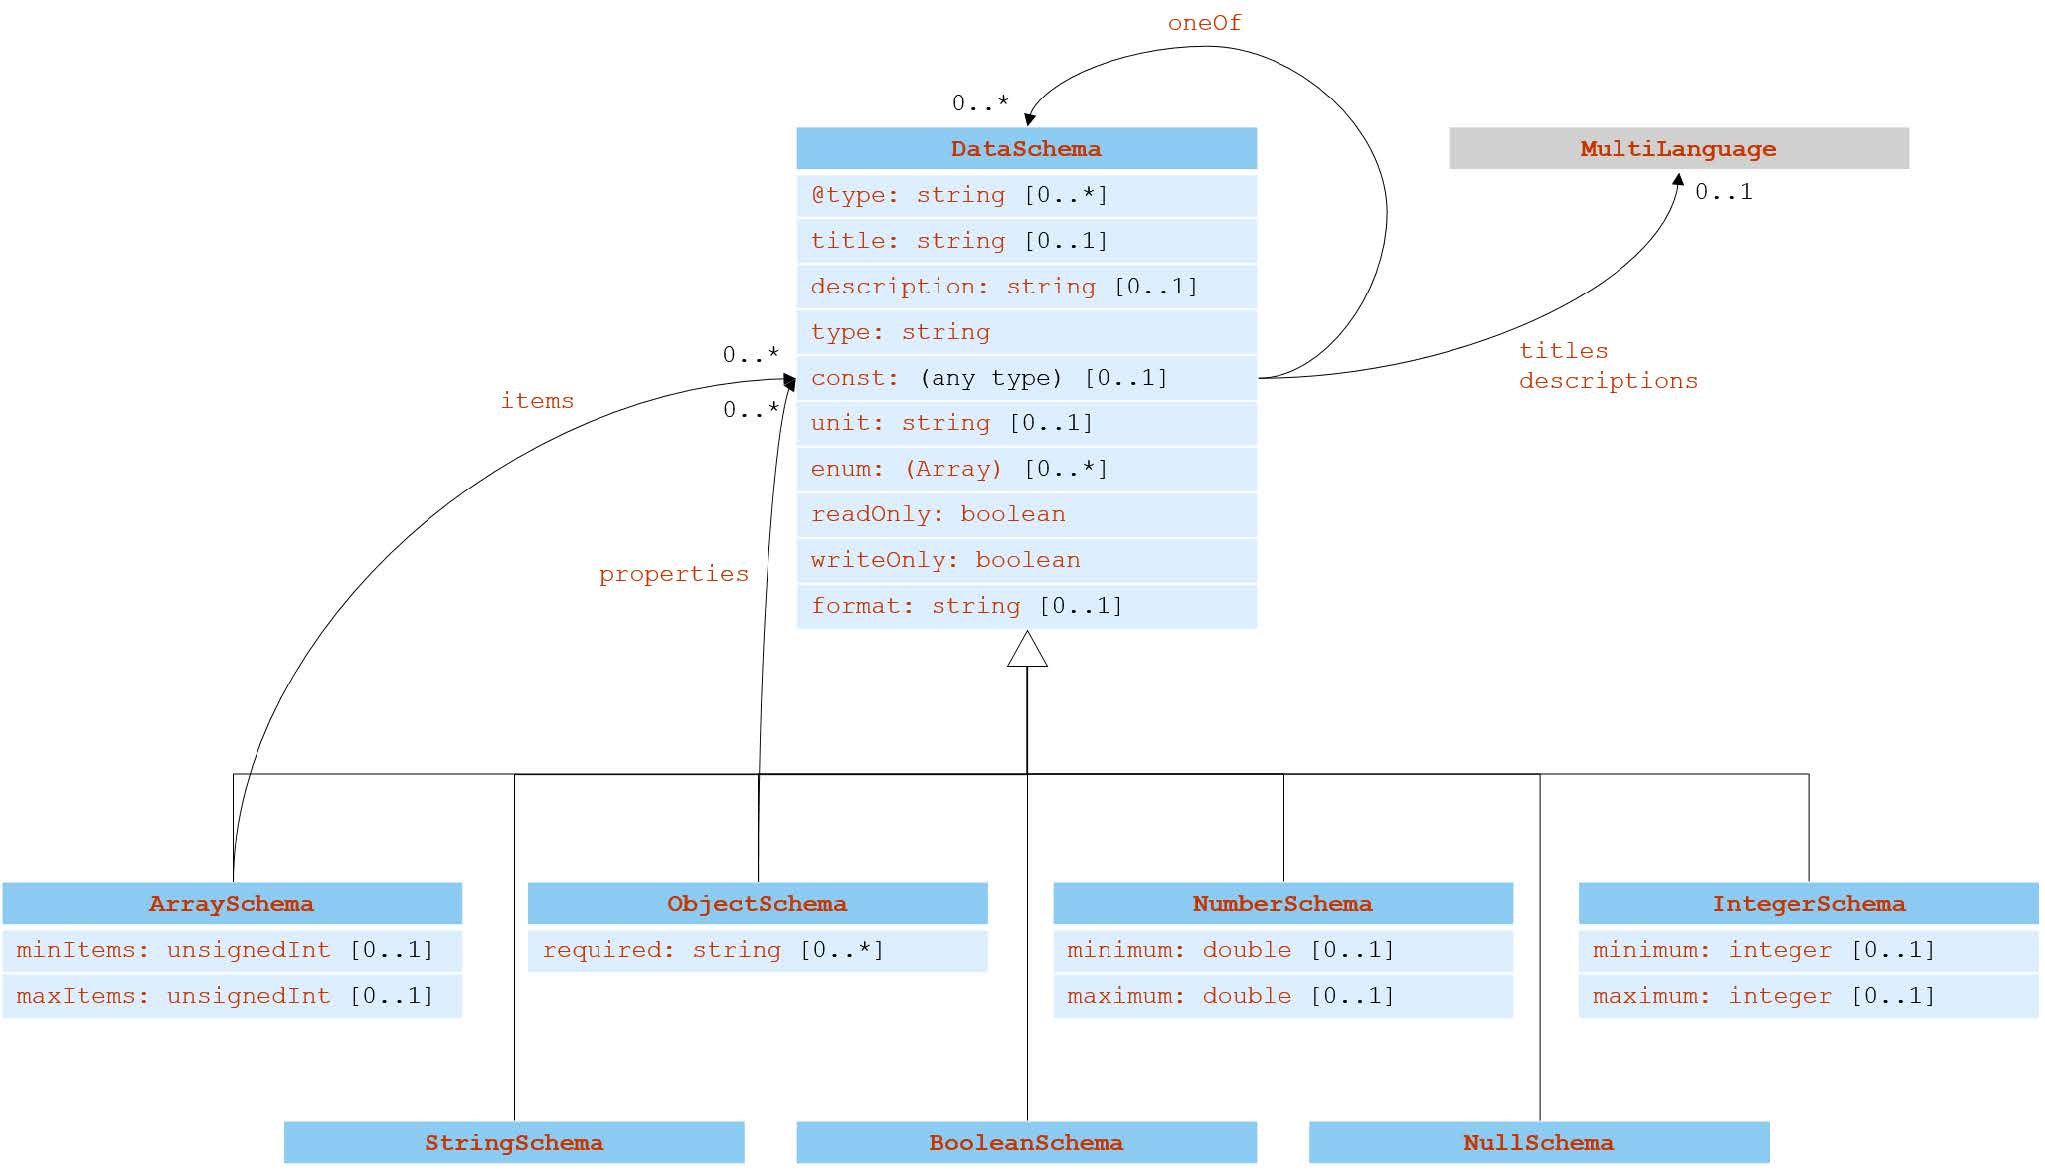
\includegraphics[width=\textwidth]{td-data-schema-vocabulary.jpg}
  \caption{\glsxtrshort{td} Datenschemavokabular}\label{fig:td_data_schema_vocabulary}
\end{figure}

\subsubsection{Sicherheitsvokabular}

Das Sicherheitsvokabular definiert Sicherheitsmechanismen und dessen Konfigurationen.

\begin{figure}[H]
  \centering
  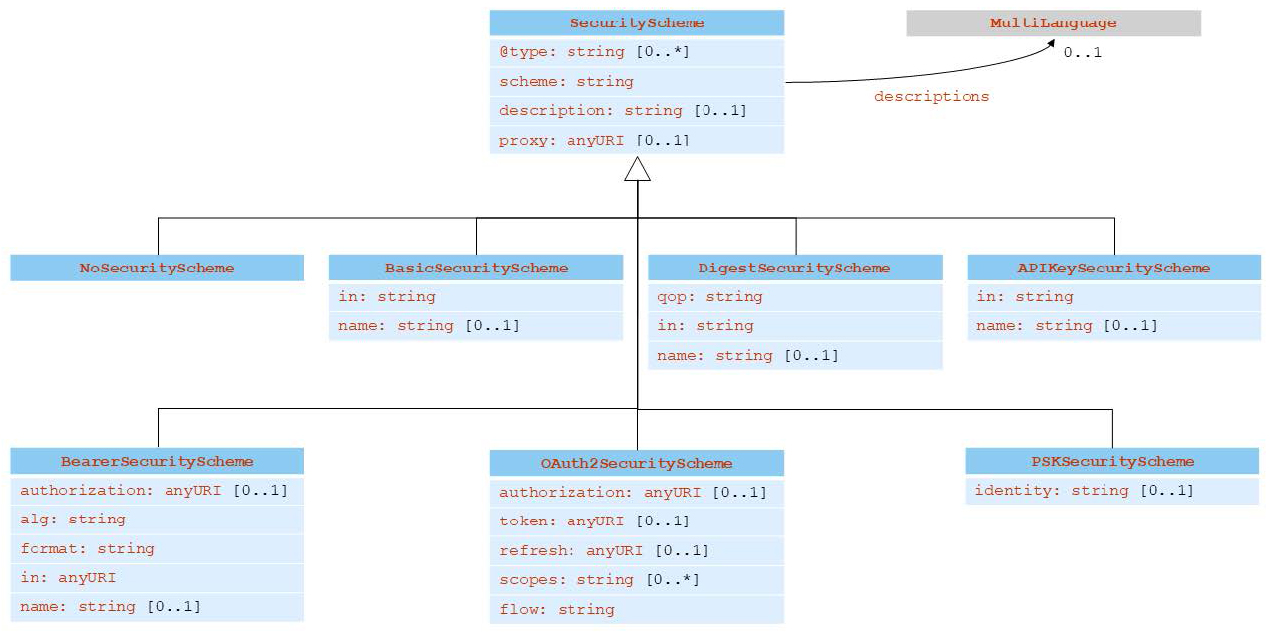
\includegraphics[width=\textwidth]{td-security-vocabulary.jpg}
  \caption{\glsxtrshort{td} Sicherheitsvokabular}\label{fig:td_security_vocabulary}
\end{figure}

Ein \lstinline{SecurityScheme} beinhaltet dabei grundsätzlich einen Bezeichner für das jeweilige Sicherheitsschema und möglicherweise Beschriftungen oder einen \glsxtrshort{uri}, auf die das Sicherheitsschema einen möglichen Zugriff definiert -- wenn es nicht um den aktuellen \glsxtrshort{uri} geht. Der Schemabezeichner wird dabei als Diskriminator für die einzelnen Sicherheitsschemata verwendet. Dabei sind je nach Sicherheitsschema weitere Objektattribute erforderlich oder möglich.

\subsubsection{Hypermediakontrollvokabular}

Das Hypermediakontrollvokabular definiert die Hauptbestandteile von Kommunikation über \gls{rest} mit Verweisen und Formularen.

\begin{figure}[H]
  \centering
  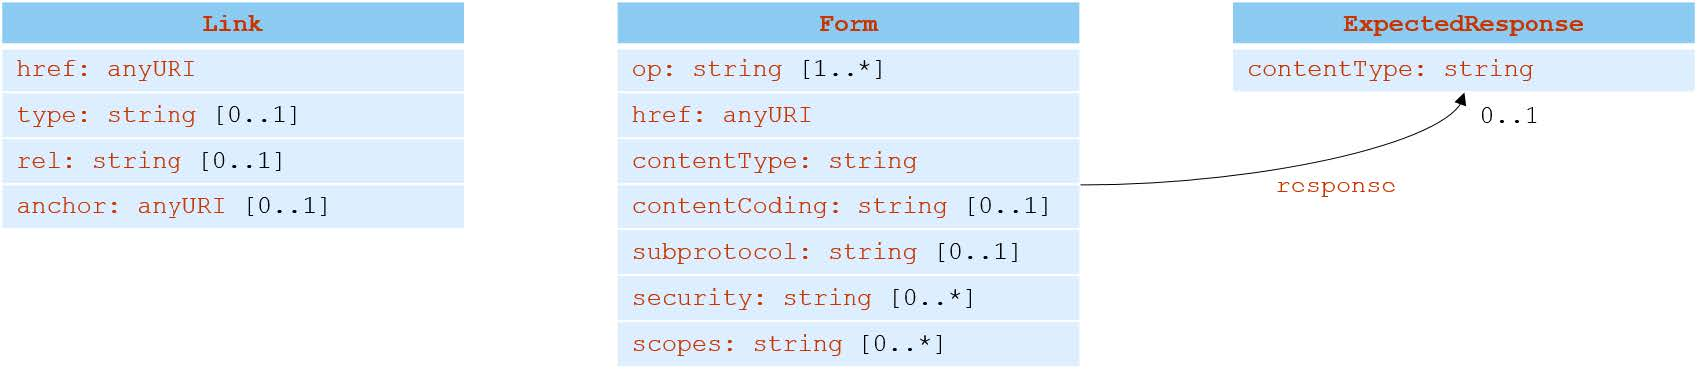
\includegraphics[width=\textwidth]{td-hypermedia-controls-vocabulary.jpg}
  \caption{\glsxtrshort{td} Hypermediakontrollvokabular}\label{fig:td_hypermedia_controls_vocabulary}
\end{figure}

\lstinline{Link}s funktionieren dabei sehr ähnlich zu Ankerelementen in \gls{html}. Sie bestehen hauptsächlich aus einem \gls{iri} und können durch den Medientyp des Ergebnisses, eine Relationsbeschreibung und einen Linkkontext erweitert werden.

\lstinline{Form}s werden an vielen Stellen verwendet. Sie bestehen hauptsächlich aus einem Bezeichner für die Operation(en), die durchgeführt werden soll(en), sowie aus einem \gls{iri}, der beschreibt, wohin das Formular geschickt werden soll. Es können noch weitere Werte ergänzt werden, wie die Art und Codierung des Inhalts, das verwendete Subprotokoll, Sicherheitsaspekte oder die Art der Antwort.
